\documentclass{artifacts/design}
    %
    % Einstellungen der Schriftart
    %
    \usepackage[T1]{fontenc}
    \usepackage[light,math]{iwona}
    
    % 
    % Blindtext zum Testen von Textausgaben
    %
    \usepackage{blindtext}    
    \usepackage{titlesec} 
    \usepackage{cite}
    \def\BibTeX{{\rm B\kern-.05em{\sc i\kern-.025em b}\kern-.08emT\kern-.1667em\lower.7ex\hbox{E}\kern-.125emX}}
    
    % 
    % Kopfzeile & Fußzeile
    %
    \pagestyle{fancy} 
    \renewcommand{\chaptermark}[1]{\markboth{#1}{}}
    \renewcommand{\sectionmark}[1]{\markright{#1}{}}
    \usepackage{etoolbox}
    
    %
    % Titelformat
    %
    \patchcmd{\chapter}{\thispagestyle{plain}}{\thispagestyle{fancy}}{}{}
    \titlespacing{\chapter}{0pt}{0pt}{0pt}
    \definecolor{gray75}{gray}{0.75}
    \newcommand{\hsp}{\hspace{20pt}}
    \titleformat{\chapter}[hang]{\Huge\bfseries}{\thechapter\hsp\textcolor{gray75}{|}\hsp}{0pt}{\Huge\bfseries}

    %%%%%%%%%%%%%%%%%%%%%%%%%%%%%%%%%%%%%%%%%%%%%%%%%%%%%%%%%
    \begin{document}
    
    %
    % Titelseite
    %
    \maketitle
    
    %
    % Vorstellung / Abstrakt
    %
    \addcontentsline{toc}{chapter}{Kernthesen}
    \chead{Kernthesen}
    \input{chapters/Kernthesen}  
    \vfill  
    \pagebreak        
    \addcontentsline{toc}{chapter}{Arbeitsprozess}
    \chead{Arbeitsprozess}
    \input{chapters/Arbeitsprozess}
    \vfill  
	\pagebreak
    
    %
    % Inhaltsverzeichnis     
    \addcontentsline{toc}{chapter}{Inhaltsverzeichnis}
    %
    \inhaltverzeichnis 
    
    %
    % Inhalt
    %
    \chapter{IceCube South Pole Observatory} 

    \vspace{8pt}

    \section{Das IceCube-Projekt}

    \subsection{Was ist das IceCube-Projekt?}

    Beim IceCube-Projekt handelt es sich um ein eine Art Teleskop beziehungsweise 
    um einen (Teilchen-)Detektor. In der folgenden Ausarbeitung werden die Begriffe 
    Teleskop und Detektor synonym verwendet. Dieser Detektor dient dazu hochenergetische 
    Neutrinos zu entdecken, zu erfassen und zu erforschen. IceCube befindet sich am 
    Südpol in der Antarktis und gehört zu der Amundsen-Scott-Südpolstation. 
    Das Volumen des IceCube beträgt etwa 1$km^3$. Es befindet sich im Eis in 3000 
    Meter Tiefe. Das Projekt und die Forschung werden seit 2010 betrieben. Das 
    Neutrino wird nachgewiesen, wenn es mit dem Eis reagiert und wechselwirkt. 
    Daraus entstehen Elektronen, Myonen und/oder Tauonen, welche im Eis für 
    Lichtstrahlung sorgen. Im IceCube befinden sich Fotomultipler (dabei handelt 
    sich um extrem empfindliche Sensoren), welche die Tscherenkow-Strahlung nachweisen \cite{FAQ13}.

    \subsection{Ziele des IceCube-Projekts}

    
    Das Hauptziel des Projekts besteht darin herauszufinden wo der Ursprung der 
    kosmischen Strahlung liegt, wozu auch das Neutrino zählt. Es gibt auch Neutrinoquellen, 
    welche von der Erde stammen, diese sind jedoch energetisch niedrig und sind weniger 
    relevant für die Forschung. Man konnte bisher feststellen, dass es keine dominierenden 
    Quellen gibt und die Neutrinos von überall aus dem Weltraum kommen. Mit bestimmten 
    Messungen des Projekts werden Rechnungen durchgeführt mit dem Ziel die Quelle zu ermitteln, 
    was jedoch nicht bei jeder Messung möglich ist, 
    da hauptsächlich Messungen von atmosphärischen Prozessen gemacht werden. Diese müssen 
    dann von den gewünschten Ergebnissen getrennt werden. Außerdem versucht man die 
    sogenannten Grundlagen zu erforschen. In diesem Forschungsgebiet der Physik gibt es 
    noch viele teils grundlegende ungeklärte Fragen, wie die Frage weshalb Neutrinos 
    elektromagnetische Kräfte ignorieren und Materie nahezu ungehindert passieren können, 
    was in der Umgebung eines schwarzen Lochs passiert, wie eine Supernova explodiert, 
    woher Neutrinos stammen und viele weitere Fragen. Durch das Projekt sollen solche 
    grundlegenden Fragen beantwortet werden, damit man auf Grundlage dieser Erkenntnisse 
    weiter und tiefgreifender forschen kann \cite{FAQ13}. Ein weiteres Ziel besteht 
    darin sogenannte GZK-Neutrinos zu beweisen. Das sind hypothetische Neutrinos mit einer 
    Energie, die die Energie kosmischer Neutrinos um den Faktor 1000 übersteigen. Man geht 
    davon aus, dass diese GZK-Neutrinos durch eine Wechselwirkung der kosmischen Strahlung 
    mit der kosmischen Hintergrundstrahlung zustande kommen. Unter der kosmischen 
    Hintergrundstrahlung versteht man eine Mikrowellenstrahlung, welche seit Beginn des 
    Urknalls existiert. Allerdings ist dies erst die Theorie, die durch Messdaten begründet 
    werden soll. Das sind die eigentlichen Ziele des Projekts, das IceCube-Projekt hat neben 
    diesen Hauptzielen auch untergeordnete Aufgaben, die auch nicht zwangsläufig im direkten 
    Zusammenhang mit der Neutrinoforschung stehen müssen.  Beispielsweise lassen sich 
    Anisotropiestudien durchführen. Darunter versteht man, dass ein Prozess, der von der 
    Bewegungsrichtung abhängig ist und das Gegenteil der Isotropie ist, bei der ein Prozess 
    nicht von der Bewegungsrichtung abhängig ist. Darunter sind beispielsweise Versuche mit 
    akustischen Wellen zu verstehen. Die Anisotropiestudien finden auch bei der 
    Neutriountersuchung statt, aber nicht ausschließlich \cite{FAQ13}.

    \subsection{Aufenthalt am Observatorium}

    Zur Zeit des australischen Sommers befinden sich etwa 150 Wissenschaftler und 
    Hilfskräfte am Observatorium. Über die Winterzeit halten sich rund 40 Wissenschaftler 
    und Hilfskräfte am Observatorium auf. Einige Wissenschaftler entschließen sich auch 
    für ein komplettes Jahr an der Amundsen-Scott-Südpolstation zu bleiben und zu forschen. 
    Dabei handelt es sich auch in der Regel um zwei Physiker die ihr Physikstudium 
    abgeschlossen haben und somit schon einige theoretische als auch praktische Kenntnisse 
    erlangt haben. Diese zwei Wissenschaftler sind damit  beauftragt die Computer, die zur 
    Datenanalyse dienen, zu warten und auch weitere Daten zu sammeln. Dies stellt aber nicht 
    die einzige Aufgabe dar, denn an der Südpolstation gibt es auch wesentlich mehr Aufgaben, 
    wie zum Beispiel die Tätigkeit in der Feuerwehr. Wie man also sehen kann nicht 
    ausschließlich wissenschaftliche sondern auch allgemeine Tätigkeiten. Während den 
    Bauarbeiten des Detektors waren etwa 48 Personen dabei, die zum IceCube-Team gehören, 
    um die sicherzustellen, dass die Arbeiten nach Plan verlaufen \cite{FAQ13}.

    \section{Geschichte}

    \subsection{Bau des IceCube}

    Das angewandte Prinzip (in 1.1 beschrieben) wurde auch in einem anderen Projekt, 
    das ebenfalls dazu diente kosmische Höhenstrahlung zu untersuchen, angewendet. 
    Dabei handelt es sich um das Projekt AMANDA (Antartic Muon And Neutrino Detector Array). 
    Dieses Teleskop wurde 2009 deaktiviert, da IceCube mehr Relevanz hatte. Jedoch wurden 
    die Gelder für das IceCube-Projekt bereitgestellt, da AMANDA große Erfolge erzielte und da 
    IceCube im Wesentlichen eine Größere Version von AMANDA ist. Die Planung für das 
    IceCube-Projekt nahm 10 Jahre in Anspruch, die Bauzeit dann 6 Jahre und nach dieser 
    Zeit am 18. Dezember 2010 wurden die Bauarbeiten beendet. Der Leiter des Projekts ist 
    Francis Halzen, welcher auch bei der Entwicklung des Projekts tätig war. 
    Francis Halzen ist ein Elementarteilchen- und Astrophysiker. \\
    Noch während des Baus des Projekts wurden die ersten wissenschaftlichen Beobachtungen 
    gemacht, welche jedoch, im Vergleich zu den anderen Beobachtungen, unwichtiger sind. 
    Die digitalen optischen Module wurden nach und nach ins Eis eingelassen und mit der 
    Südpolstation vernetzt, weshalb während der Bauzeit schon Messungen durchgeführt wurden, 
    diese waren aber aus dem Grund irrelevant, da ihre Energien zu niedrig waren und eher 
    Neutrinos atmosphärischer Wechselwirkungen waren. \\
    2013 hat man die zu diesem Zeitpunkt fundamentalste Entdeckung von hochenergetischen 
    kosmischen Neutrinos gemacht. Also nach etwas mehr als zwei Jahren, was zeitlich gesehen, 
    kein langer Zeitraum ist, wenn man bedenkt, dass die Wechselwirkung zwischen Materie und 
    Neutrinos selten ist \cite{FAQ13}.

    \subsection{Erfolge}

    Durch das IceCube-Projekt gab es viele wissenschaftliche Erfolge im Bereich der 
    Astro- und Teilchenphysik. Zum einen hat die IceCube-Kollaboration im Juni 2013 
    erste Hinweise darauf veröffentlicht, dass einige Messungen darauf hindeuten, dass es einen
    Fluss von Neutrinos gibt, der auf eine unbekannte Strahlungsquelle hindeutet, wie einer möglichen 
    Supernova. Jedoch gab es nur wenige Messwerte, weshalb man noch keine empirisch belegte Aussage treffen konnte. 
    Diese Hinweise, die zu dieser Hypothese geführt haben, wurden im November 2013 bestätigt. 
    Am IceCube-Projekt wurden weitere Messungen durchgeführt, die die Hypothese bestätigt 
    haben und gezeigt haben, dass das Neutrino nicht terrestrisch ist, das bedeutet, dass es
    nicht von der Erde ausgeht. Für diese Erkenntnis verlieh das Magazin \grqq Physics World\grqq{}
    den Preis \grqq Breakthrough of the year 2013\grqq{}. Man konnte außerdem den Nachweis
    für die Existenz von kosmischen Myonneutrinos erbringen.\\
    Zwischen dem Mai 2010 und dem Mai 2012 hat man 28 Ergebnisse gemessen mit 
    hochenergetischen Neutrinos. Darunter 1000; 1100 und 2200 Tesla-Elektronenvolt. 
    Außerdem hat man ein Neutrinoereignis mit einer Energie von 2600 TeV (Elektronenvolt) 
    messen können, was die bisher größte gemessene Energie bei den Neutrinos darstellte. 
    Die Messung mit 2200 Tesla-Elektronenvolt wird als Big Bird deklariert. Ein möglicher Ursprung 
    der Strahlung Big Bird konnte ermittelt werden durch einen Vergleich der Versuchsdaten vom 
    IceCube-Projekt mit den Daten des Gammastrahlen-Weltraumteleskop Fermi und mit dem 
    Radioteleskop Tanami. Die Wissenschaftler, die mit diesen Teleskopen beauftragt sind, 
    wurden nach der Entdeckung diese Ereignis konsultiert und richteten mithilfe der 
    IceCube-Daten die Teleskope neu aus. Dabei handelt es sich um einen Blazar-Ausbruch in 
    der Galaxie PKS B 1424-418, welcher für kosmische Höhenstrahlung sorgt. Dies stellt 
    jedoch nicht die einzige gefundene Quelle von Neutrinos dar. Bei einem weiteren Vergleich 
    mit anderen Teleskopen konnte man einen aktiven Galaxiekern identifizieren, welcher ein 
    möglicher Ursprung von hochenergetischen Protonen ist, was zumindest vermutet wird. Ein 
    noch aktuelleres Ergebnis konnte man 2018 registrieren als man Daten von IceCube mit den 
    Daten von anderen Teleskopen verglichen hat und den Blazar TXS 0506+056 als potentielle 
    Quelle ausmachte und nicht nur für Neutrinos sondern auch für hochenergetische Protonen \cite{FAQ13} \cite{DeFuInt18}.
    
    \newpage
    
    \section{Konstruktion und Technik}

    \subsection{Aufbau des Detektors}

    \begin{center}
        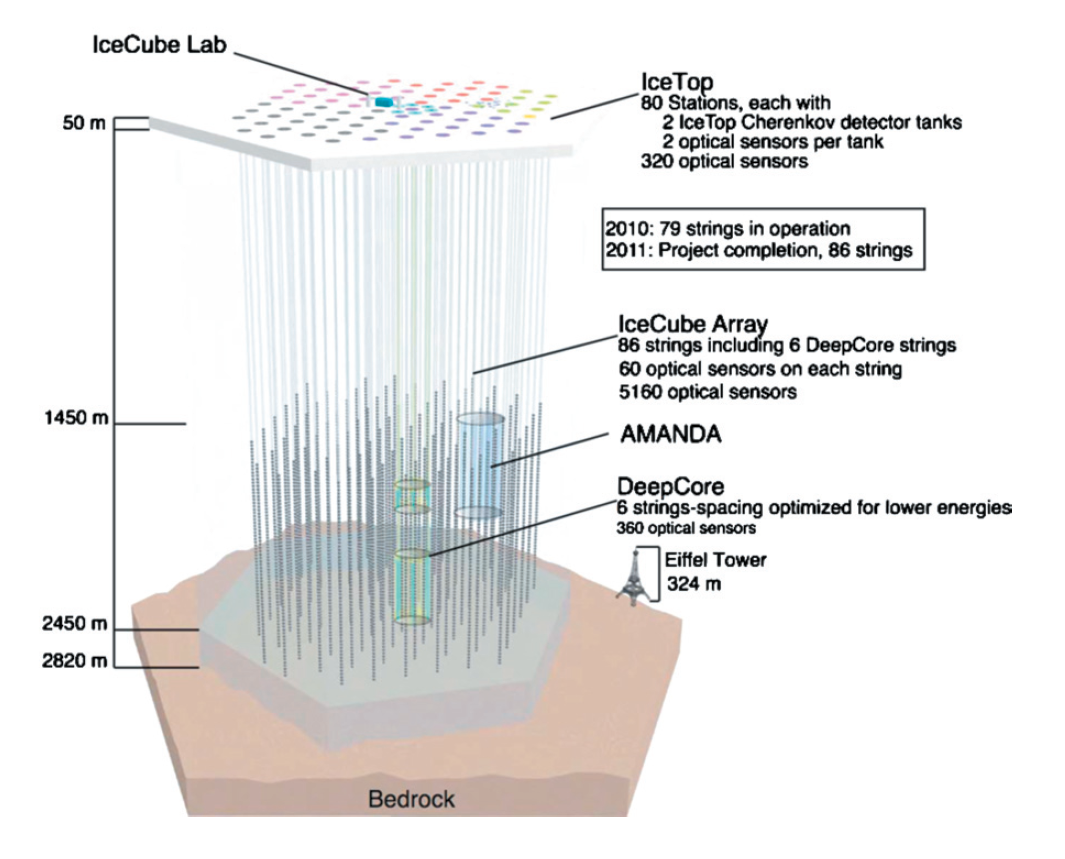
\includegraphics[scale=0.42]{images/architeture.png} \\
        Quelle: IceCube Science Team - Francis Halzen, Department of Physics, University of Wisconsin      
    \end{center}

    \newpage

    \subsection{Funktionsweise der Bestandteile}

    \begin{wrapfigure}{r}{0.25\textwidth}
        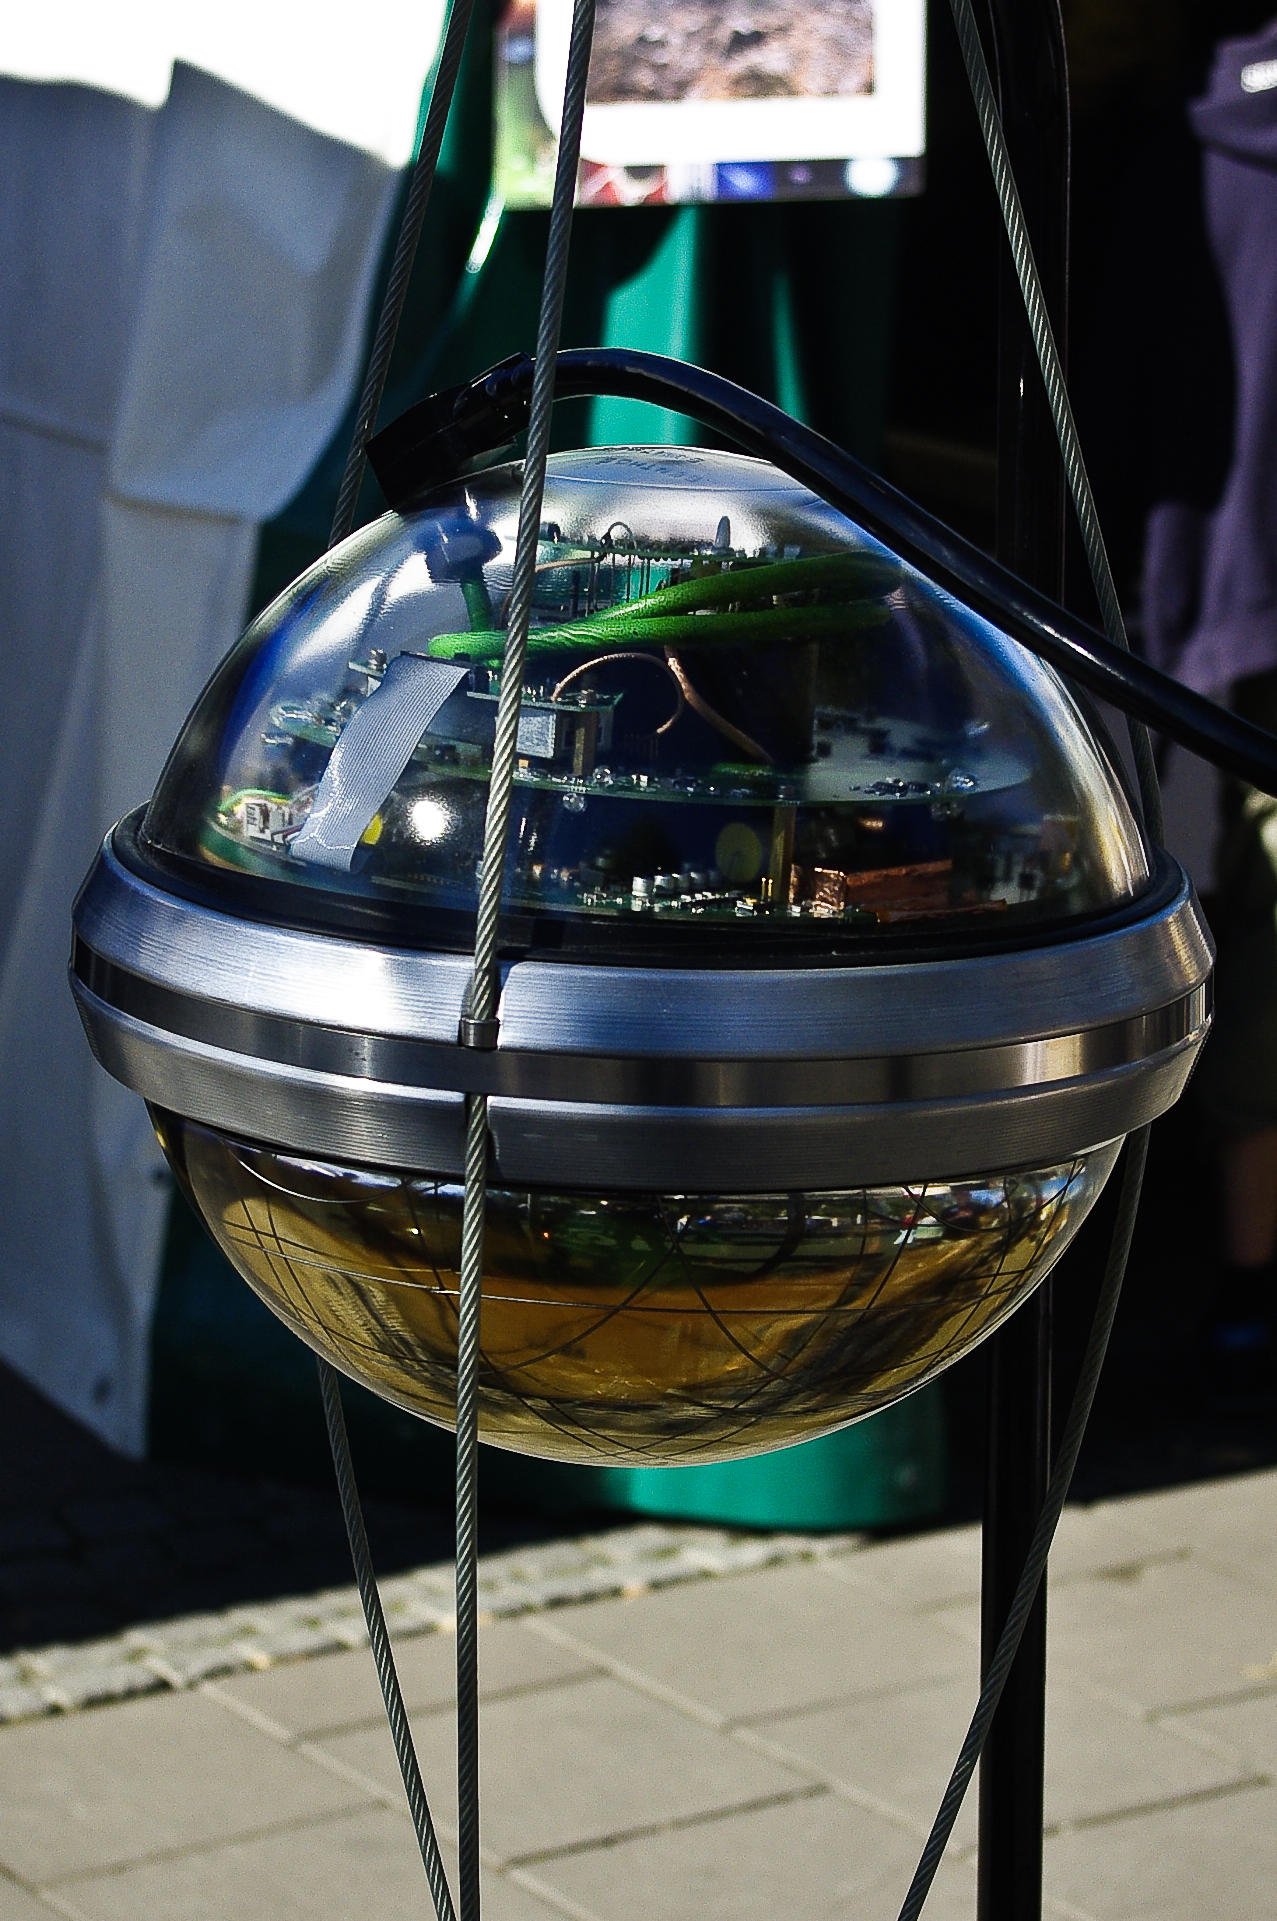
\includegraphics[width=0.24\textwidth]{images/pmt.jpg}
        Quelle: Taavi Adamberg
    \end{wrapfigure}  

    Im oberen Bild kann man den Aufbau des Detektors erkennen. 
    Im Eiswürfel befinden sich 5160 der digitalen optischen Module (Akronym: DOMs/Bild auf der rechten Seite) 
    mit jeweils einem Photomultipler und der notwendigen Elektronik. Der Photomultiplier 
    (oder auch Photoelektronenvervielfacher) dient dazu die schwachen Lichtsignale 
    (beispielsweise der Photonen oder Myonen) zu verstärken durch die Erzeugung eines elektrischen Signals, 
    welcher nun die Messung verstärkt. Damit möglichst viele Ergebnisse gesammelt werden können liegt der 
    Empfangsbereich zwischen 300 und 650 nm. Die Funktion der DOMs besteht darin die Tscherenkow-Strahlung 
    zu registrieren, sie zu verstärken, zu digitalisieren und sie an die Station weiterzuleiten. 
    Die DOMs sind an vertikal positionierten \grqq Saiten\grqq{} befestigt. Die Anordnung ist regelmäßig. 
    Der Abstand zwischen den einzelnen Saiten und DOMs ist immer gleich außer im DeepCore Unterdetektor, 
    denn dort gibt es eine dichtere Anordnung der Saiten und DOMs, um Neutrinooszillationen messen zu können, 
    da so die Energieschwelle der Neutrinos heruntergesetzt wird auf etwa 10 GeV. 
    Die DOMs sind zusätzlich noch mit einem eigenen Mini-Computer sowie einer Präzisionsuhr ausgestattet. 
    Die Präzisionsuhr misst auf etwa 5 Nanosekunden genau, wann das Tscherenkow-Licht registriert wird, 
    um bessere Berechnungen und Datenanalysen durchführen zu können. 
    Diese Daten werden dann über kilometerlange Kabel zu dem Datenerfassungssystem in der Südpolstation 
    weitergeleitet. \\
    Über dem Detektor befindet sich das sogenannte IceTop mit 81 Stationen. Die Stationen befinden sich 
    hauptsächlich über den Saiten und sind mit jeweils zwei Tanks ausgestattet, die ebenfalls zwei DOMs haben, 
    die nach unten ausgerichtet sind. IceTop dient ebenfalls dazu Höhenstrahlung zu messen, aber IceTop wird 
    vorwiegend dazu verwendet, um die Zusammensetzung der Höhenstrahlung  zu identifizieren und IceTop hilft 
    dabei die Richtung des Elementarteilchenflusses zu bestimmen. Des Weiteren kann man auch Messungen erfassen 
    von Primärstrahlung über \grqq Luftduschen\grqq{} , das heißt, dass auch oberhalb des Eises kosmische Höhenstrahlung 
    gemessen werden kann. Die ist ein kleiner Forschungsaspekt, der vor allem als Vergleich und Abgleich dient. 
    Myonen können auch durch Wechselwirkungen von Höhenstrahlung mit der irdischen Atmosphäre entstehen. 
    Man möchte mit IceCube Daten aussortieren, die aus atmosphärischen Prozessen entstehen. 
    Wenn nun also IceCube ein Ergebnis registriert und dieses zusammenfällt mit IceTop, dann kann man davon 
    ausgehen, dass diese Daten eine atmosphärische Quelle haben und man muss sich nicht weiter damit 
    auseinandersetzen, was die Datenanalyse erleichtert. \cite{BachJoHa}
    Oftmals erfassen die optischen Module sogenanntes Hintergrundrauschen, von beispielsweise Photonen. 
    Diese Daten müssen dann aussortiert werden. Oftmals kann man solche Daten schon aussortieren, wenn man 
    erkennt, dass ihre Energien in einem niedrigen Bereich liegen. \cite{DESY16}

    \subsection{Instandhaltung der Sensoren}

    Wie bereits angesprochen besteht der Detektor zu einem großen Anteil aus Sensoren, 
    die die Tscherenkow-Strahlung identifizieren. Sobald sich die Sensoren im Eis befinden kann man sie 
    physisch nicht mehr erreichen, deshalb werden sie sorgfältig geprüft und getestet werden, 
    bevor sie eingesetzt werden. Denn nachdem die Module ins Eis eingelassen wurden, wurden diese 
    Stellen wieder zugefroren und IceTop wurde oberhalb des Detektors errichtet. Es ist jedoch möglich 
    auf die Software des Sensors zuzugreifen und ein Software Remote zu starten, wenn es beispielsweise 
    elektronische Probleme gibt, denn alle Sensoren sind mit dem IceCube Lap am Südpol verbunden. IceCube 
    Lap meint die Computer, die mit den DOMs verbunden sind. \cite{FAQ13}

    \section{Funktionsweise und Messungen}

    Mit dem Teilchendetektor werden an sich keine Neutrinos registriert sondern sogenannte Sekundärteilchen. 
    Wenn ein Neutrino auf das Eis trifft, kommt es selten zu Wechselwirkungen, in Form von einem Neutrino, 
    das auf ein Proton oder Elektron eines Atoms stößt und eine Kernreaktion in Gang setzt. Aber wenn diese 
    sogenannte schwache Wechselwirkung zustande kommt, dann entstehen daraus Sekundärteilchen wie Elektronen, 
    Myonen oder Tauonen, welche dann vom Detektor gemessen werden. Im Fall, dass man die gewünschten Ergebnisse 
    erzielt gilt es vor allem die Richtung dieser zu bestimmen. Ideal für diese Bestimmung ist es, wenn ein 
    Myon-Neutrino mit einem Eismolekül wechseltwirkt. Aus dieser Wechselwirkung entstehen dann Myonen. 
    Ein Myon behält idealer Weise die Bewegungsrichtung des Neutrinos bei auch nach der Wechselwirkung mit Eis. 
    Dieses Myon durchquert die Sensoren und hinterlässt dabei blaues Licht, die Tscherenkow-Strahlung. 
    Unter Tscherenkow-Strahlung versteht man im weitesten Sinne eine bläuliche Lichterscheinung, die entsteht, 
    wenn relativistische und geladene Teilchen wie beispielsweise Myonen oder Tauonen durch ein Dielektrikum 
    gehen. Die entstehenden Lichtblitze werden durch Fotomultipler verstärkt und die Lichtstrahlung wird dann 
    in elektrische Impulse umgewandelt. Diese Messdaten kann man dann im Hinblick auf die Bewegungsrichtung 
    auswerten und anhand der Ankunftszeiten der Teilchen bei den Sensoren oder den Eintrittswinkeln, lässt 
    sich dann die Bewegungsrichtung berechnen. Diese Berechnungen sind äußerst präzise mit einer Ungenauigkeit 
    des Eintrittwinkels von $0,5^\circ$. Es wird sich zu Nutze gemacht, dass sich die Neutrinos ungehindert und 
    geradlinig durch das Weltall bewegen, da sie elektrisch neutral sind und somit nicht durch Magnetfelder 
    abgelenkt werden können. Des Weiteren findet eine Wechselwirkung mit Materie eher selten statt, somit 
    behalten sie auch ihre Flugbahn auf der Erde bei und auch nach der Wechselwirkung mit dem Eis bleibt die 
    Bewegungsrichtung dieselbe, zumindest bei den Myonneutrinos. Dies war ein ausschlaggebender Grund weshalb 
    sich das IceCube-Team vorwiegend auf Myonneutrions fokussierte. Auch deshalb, weil die Lichtblitzte, 
    die sie erzeugen, sich über Kilometer erstrecken können und somit trotzdem den Detektor durchlaufen. 
    So können auch Wechselwirkungen registriert werden, welche eine größere Distanz zum Detektor haben. 
    Somit kann man beim Eintreffen auf der Erde leichter Rückschlüsse ziehen und Berechnungen zu ihrem 
    Ursprung durchführen. Allerdings werden auch die anderen Neutrinoarten untersucht, da man einige Daten 
    gesammelt hat, welche nicht durch die Wechselwirkung eines Myons mit Eis zustande kamen. \\
    Die kosmische Höhenstrahlung besteht aus vielen geladenen Teilchen wie Protonen und erstmal keinen 
    Neutrinos. Diese Höhenstrahlung würde durch das Magnetfeld abgelenkt werden und man könnte so keinen 
    Rückschlüsse ziehen, aber man geht davon aus, dass die kosmische Höhenstrahlung an ihrem Ursprungsort 
    mit Photonen wechselwirkt und daraus Neutrinos entstehen. \\
    Damit die Neutrinos Licht erzeugen können, gilt folgende Gleichung:
    \begin{center}
        $Geschwindigkeit>\frac{Lichtgeschwindigkeit}{Brechungsindex} = v >\frac{u}{n}$
    \end{center}
    Nach dieser Formel muss also die Geschwindigkeit der Neutrinos, nach der stattgefundenen 
    Wechselwirkung mit dem Medium, größer sein als der Quotient aus Lichtgeschwindigkeit und des 
    Brechungsindex des Mediums (beispielsweise Eis). Dies lässt sich auch in einer Rechnung verdeutlichen:
    \begin{center}
        $228850050\frac{m}{s}>\frac{299792458\frac{m}{s}}{1,31}=228849204,58\frac{m}{s}$
    \end{center}
    Der Quotient ist kleiner als die Geschwindigkeit des Neutrinos, was nun die Registrierung des 
    Lichts mit dem Detektor ermöglicht. Damit man diese Rechnung überhaupt anwenden kann gilt, 
    dass die Neutrinos nicht nur das Medium durchqueren sondern auch mit ihnen wechselwirken. \\
    Es entsteht ein sogenannter \grqq Überlichtknall\grqq{}, dieser ist an der Tscherenkow-Strahlung bemerkbar. \\
    Ein weiterer wichtiger Aspekt ist ebenfalls, dass man Neutrinos nie direkt nachweisen kann, 
    da sie elektrisch neutral sind, weshalb man sie lediglich über die Sekundärteilchen nachweisen kann, 
    die sie durch Wechselwirkung hinterlassen. \cite{IcePhyCos13} \cite{SdW16} \cite{WdP13}\\
    Die Reaktion im Eis läuft nach folgender Gleichung ab:
    \begin{center}
        $\nu_\mu+N\rightarrow\mu$
    \end{center}

    \section{Warum befindet sich das Projekt am Südpol ?}
    
    Elementar zu beantworten ist, weshalb sich das Projekt am Südpol und nicht beispielsweise am 
    Nordpol oder in Amerika in Wisconsin befindet. Dafür gibt es viele Gründe. Ein wichtiger Grund, 
    warum sich das Projekt an einem der beiden Pole befinden muss ist, dass wie bereits angesprochen 
    die Neutrinos mit dem Eis wechselwirken und die dadurch entstehenden Teilchen (im Folgenden als 
    Sekundärteilchen bezeichnet), Licht abgeben und die Detektoren des IceCube registrieren dies als 
    Tscherenkow-Strahlung bezeichnete Licht. Das Licht wird teilweise bis zu einem Kilometer erstreckt, 
    somit werden viele Eisatome gebraucht, damit IceCube es registrieren kann. Damit dieser Prozess effektiv 
    ablaufen kann benötigt man große Mengen an einem transparenten Material, wie in diesem Fall Eis, da die 
    Wechselwirkung zwischen dem Eis und den Neutrinos eher selten ist. \\
    Ein Vorteil am Südpol im Gegensatz zum Nordpol ist, dass der Südpol viel Eis enthält mit den Eigenschaften, 
    dass es klar, rein sowie stabil ist was eine optimalere Wechselwirkung der Höhenstrahlung mit dem Eis 
    ermöglicht. \\
    Des Weiteren enthält Eis Luftblasen, welche die Messungen von IceCube verfälschen würden, 
    da das Medium ein anderes wäre, in welchem sich das Licht ausbreiten würde beziehungsweise würden 
    weniger Wechselwirkungen stattfinden, nicht zu vergessen ist, dass die Detektoren auch somit viel
    mehr uninteressante Messungen registrieren würden und das Licht seine Geschwindigkeit und Richtung 
    verändern würde. Jedoch ist dies am Südpol nicht so stark ausgeprägt, da sich am Südpol mit der Zeit 
    Eis und vorwiegend Schnee auftürmten, und zwar sehr dick und dicht, so wurden die darunterliegen 
    Eisschichten nach unten gedrängt, zusammengedrückt und komprimiert. Der Druck verdrängte die Luftblasen. 
    Man spricht davon, dass das tiefe Eis am Südpol ultra-transparent ist. \\
    IceCube muss abgeschirmt werden, um es vor Strahlung an der Erdoberfläche zu schützen, da diese 
    die Messwerte verfälschen würden. Die Sensoren von IceCube beginnen erst ab einer Tiefe von 1500 
    Metern und liegen somit geschützt vor der natürlichen Einstrahlung an der Erdoberfläche. Man muss 
    auch bedenken, dass die IceCube-Kollaboration trotzdem noch Messungen von Strahlungen atmosphärischer 
    Herkunft macht. Wenn nicht, dann gäbe es eine Überflutung mit irrelevanten Daten. Außerdem bietet 
    sich H2O (ob flüssig oder gefroren) an, da es ein transparentes  Element ist. Dieses Element bietet 
    den Vorteil, dass es dieses Element zur Genüge gibt. Ein anderes Experiment zum Neutrinonachweis 
    benötigte Gallium, was seltener und teurer ist. Dies sind alles Anforderungen, die für Durchführung 
    des IceCube-Projekts erfüllt sein müssen. Die Südpolstation, wo sich das IceCube befindet, befindet 
    sich an einem Ort in der Antarktis, an der alle diese Bedingungen und Anforderungen zum Großteil 
    gegeben sind \cite{FAQ13}.

    \section{Wie wichtig ist das IceCube-Projekt und hat es einen Nutzen?}

    Wie bereits angesprochen handelt es beim IceCube-Projekt um Grundlagenforschung durch welche man sich 
    erhofft noch mehr Informationen zu sammeln mit denen man sich vieles erklären kann. In diesem Fall 
    geht es um unser Universum. Wenn die Grundlagen verstanden werden, kann man mit diesen viele übergeordnete 
    Dinge erklären und diese helfen dabei das Universum zu studieren. Die Neutrinos werden mit Fingerabdrücken 
    verglichen, welche ein Hinweis auf etwas Größeres sind. \\
    Im Hinblick darauf hat das Projekt eine große Relevanz. Zum einen da man mit dem IceCube-Projekt schon 
    erste Erfolge erzielte und diese Erfolge stellen einen Schritt in die Beantwortung der Fragen dar. 
    Beispielsweise besteht unser Universum zu etwa 4\% aus Materie, dazu gehören Atome und die dazugehörigen 
    Elektronen aber auch Protonen. Dann gibt es auch die dunkle Materie, die etwa 23\% unseres Universums 
    ausmacht und die dunkle Energie (etwa 73\%). Über dunkle Materie und dunkle Energie ist nur sehr wenig 
    bekannt und die Forschung über Neutrinos hilft dabei die dunkle Materie und Energie zu erforschen und zu 
    erklären. Dies ist nur ein Beispiel, es gibt noch weitere Bereiche und Phänomene, die man mit den 
    Ergebnissen der Neutrino-Forschung erklären möchte beziehungsweise versuchen wird. Ein anderer 
    Forschungsaspekt ist die allgemeine Relativitätstheorie. \\
    Des Weiteren führen neue Erkenntnisse zu weiteren Erkenntnisse was zu einer Kausalitätskette führt 
    und je mehr Erkenntnisse die Menschen erlangen desto mehr Fortschritt kann es geben von dem alle 
    Menschen profitieren können \cite{FAQ13}.

    \section{Verbesserungsmöglichkeiten des IceCube-Projekts}

    Da sich das Konzept des IceCube-Projekts schon als funktionierend herausgestellt hat muss man dort 
    keine Veränderungen vornehmen. Um die Messungen zu verbessern müsste man den gesamten Detektor vergrößern, 
    da dies die Wahrscheinlichkeit erhöht eine Messung einer Wechselwirkung zu machen, denn auch an Stellen 
    ohne Detektor finden logischerweise Wechselwirkungen zwischen Neutrinos und dem Eis statt. Natürlich ist 
    es nahezu unmöglich dies durchzuführen, da dies Unsummen an Geldern beanspruchen würde, die einfach nicht 
    zur Verfügung stehen, da finanzielle Mittel auch an anderen Stellen der Forschung, sei es Astrophysik oder 
    Kernphysik, benötigt werden. Ansonsten ist es schwierig das IceCube-Projekt zu verbessern. Bei der Analyse 
    der Daten sollte darauf geachtet werden, dass man die Daten mit den Daten anderer Teleskope miteinander 
    vergleicht und die Daten nach ausgewählten Analyseaspekten auswertet. Des Weiteren sollte man stets auf 
    Anomalien achten, die einen möglichen Hinweis auf eine neue Entdeckung darstellen. Dies wurde auch 
    beispielswiese bei IceCube angewandt. Durch einen Vergleich mit dem Teleskop \grqq Fermi\grqq{} und einer neuen 
    Ausrichtung dieses konnte man den wahrscheinlichen Ursprung einer Neutrinoquelle lokalisieren. IceCube 
    sollte also auch auf Zusammenarbeit setzen. Diese Analysemethode wird vermutlich schon effektiv 
    durchgeführt, da sich viele erfahrene Wissenschaftler mit den Daten auseinandersetzen und die 
    Erfolge für eine effektive Forschung sprechen. \\
    An den Photomultiplern wird auch derzeit gearbeitet, um die Messungen genauer zu gestalten, dafür gibt 
    es auch konkrete Pläne (Näheres bei 1.9). Dadurch sollen unter anderem mehr Daten gesammelt werden. 
    Eine weitere Möglichkeit den Detektor zu verbessern besteht darin mehr Foschungsaspekte zu entwickeln, 
    die man alle mit dem IceCube-Projekt abdecken kann. Dabei muss es nicht nur um Neutrinoforschung gehen, 
    sondern kann das Spektrum an Forschungsgebieten auch auf andere Gebiete der Naturwissenschaft erweitern. 
    Beispielsweise kann man das IceCube-Projekt auch für den Nachweis magnetischer Monopole verwenden, 
    beziehungsweise lässt sich der Detektor bei der Forschung anwenden. Des Weiteren lassen sich eventuell 
    akustische Sensoren entwickeln, denn bisher wurden ausschließlich optische Sensoren eingesetzt. Mit 
    zusätzlichen akustischen Modulen wird eine gewisse Menge an Vergleichsmaterial geboten und eventuell 
    bietet diese Module eine höhere Empfindlichkeit. Dies müsste sich aber erst praktisch zeigen \cite{DaAn18}.

    \section{Gescheiterte PINGU-Erweiterung}

    Diese Erweiterung war bereits Ende 2013 geplant, wurde jedoch abgelehnt, da die Erweiterung eine sehr 
    hohe Geldsumme in Anspruch genommen hätte. Das Akronym PINGU steht für \grqq Precision IceCube Next Generation 
    Upgrade\grqq{} und stellt, wie der Name vermuten lässt, eine Erweiterung des IceCubes dar. 
    Wie bereits widerlegt wurde, besitzen Neutrinos, entgegen der ursprünglichen Annahme, eine Masse. 
    Jedoch weiß man nicht, welche Masse genau ein Neutrino hat. Bisher ist man lediglich im Stande zu sagen, 
    dass die Masse eines Neutrinos kleiner als < 4·10-36 kg ist. Mit PINGU soll die genaue Masse bestimmt 
    werden beziehungsweise die sogenannte Neutrinomassenhierarchie, wodurch man die Neutrinos nach ihrer Masse 
    ordnen kann. Dies soll über die Messungen von Neutrinooszillationen geschehen. Die Konstruktion dieser 
    Erweiterung war vergleichbar mit dem DeepCore-Bereich des IceCubes. Es sollte ebenfalls einen 
    Energieschwellenwert von etwa 10 GeV haben, um möglichst viele Oszillationen messen zu können. 
    PINGU sollte jedoch größer werden als der DeepCore-Bereich des IceCubes. Auch die optischen Module 
    sollen nahezu den gleichen Aufbau haben wie die Module im IceCube-Projekt. Dazu gehört der Behälter, 
    die Photomultipler als auch die restliche Technik, bis auf die Moduleltronik. Diese muss verändert 
    werden, da einige Bestandteile veraltet sind. Die Software müsste ebenfalls leicht verändert und 
    an die Forschung angepasst werden, jedoch nicht zu stark, da sich die Forschungen ähneln und PINGU 
    im Prinzip ein verbesserter DeepCore-Detektor ist. Neben der Bestimmung der Neutrinomassenhierarchie, 
    gab es wesentlich mehr Ziele, die nicht unbedingt mit Astrophysik zu tun haben, aber durch die 
    Forschungsergebnisse zu den Neutrinos zu erklären sind. Diese Ziele sind jedoch erst dann 
    zu erreichen, wenn die Massen der einzelnen Neutrinos geklärt sind, doch als erstes gilt 
    es zu bestimmen wie sich die atmosphärische Höhenstrahlung zusammensetzt. Mit der K
    onstruktion eines solchen Detektors erhöht sich die Empfindlichkeit und man kann mehr 
    Rückschlüsse über die Neutrinooszillationen ziehen und zu welchem Anteil die kosmische 
    Höhenstrahlung aus Neutrinos besteht. Trotzdem gilt PINGU als eine Erweiterung von IceCube, 
    die sich vor allem auf niedrige Energien konzentriert. Dies sind dann vor allem Messungen 
    von beispielsweise solaren oder atmosphärischen Neutrinos, aber auch von Neutrinos, die einen 
    komplett anderen Ursprung haben. PINGU stellt ein Langzeitprojekt dar. Vermutungen der Kollaboration 
    besagen, dass etwa nach einem Jahr die Mischparameter der atmosphärischen Höhenstrahlung ermittelt 
    werden könnte. Nach zwei weiteren Jahren solle man dann in der Lage sein den drei Neutrinoarten 
    ihre definierte Masse zuordnen zu können. Innerhalb von 10 Jahren geht man davon aus, dass man die 
    Zusammensetzung des Erdkerns ermitteln könne. Man würde Rückschlüsse ziehen über die verschiedenen 
    Quellen und von woher sie stammen. Neutrinooszillationen, die zuerst den Erdkern passieren, werden 
    eventuell von den Elektronen abgehalten, wenn es zu einer schwachen Wechselwirkung kommt. 
    Diese Daten kann man dann abgleichen mit den erhobenen Daten, deren Teilchen nicht vorher den 
    Erdkern passierten. Dafür muss eine Versuchsreihe angesetzt werden, da man empirisch belegte 
    Aussagen nur treffen kann, wenn man genügend Daten gesammelt hat. Außerdem findet eine 
    Wechselwirkung mit dem Erdkern selten statt, denn dort tritt wieder das Problem auf, 
    dass Neutrinos nur selten wechselwirken. Dadurch kann man die Elektronendichte im Erdkern 
    bestimmen und darüber lassen sich Aussagen über die chemische Zusammensetzung treffen. 
    Genauer gesagt welche Elemente sich zu welchem Anteil im Erdkern befinden. \\
    Vermutlich stellt diese lange Zeitspanne einen weiteren Grund dar, weshalb der Bau nicht mit 
    Fördergeldern subventioniert wurde. Zu dieser langen Forschungszeit muss noch ein Zeitraum der 
    genauen Konstruktion und des Baus hinzu gerechnet werden. \\
    In diesem Zeitraum wird es eventuell auch andere Forschungsteams geben, die sich mit der 
    Ermittlung der Masse beschäftigen oder auch mit der Zusammensetzung des Erdkernes. 
    Außerdem ist es wahrscheinlich schwierig die genaue Zusammensetzung des Erdkerns zu bestimmen, 
    da man wahrscheinlich viel mehr Daten benötigte als man in dieser Zeit sammeln könnte. 
    Darüber hinaus ist es schwierig dadurch die genaue Zusammensetzung zu erfahren, da unterschiedliche 
    Elemente ähnliche Eigenschaften aufweisen wie sie mit Neutrinos interagieren und man nicht genau 
    sagen kann um welche Elemente es sich handelt. Die Pläne für PINGU stehen jedoch immer noch und sind 
    nicht verworfen und es wird geplant IceCube damit zu erweitern, denn möglicherweise werden die 
    Forschungsgelder noch genehmigt \cite{DaAn18} \cite{PinMar14} \cite{PINGU13}.

    \section{Zukunft des IceCube-Projekts}

    Zum jetzigen Zeitpunkt befindet sich das Projekt nun etwa 8 Jahre in Betrieb und es gab viele 
    Messungen und Beobachtungen, die für die Astroteilchenphysik wichtig waren.  Marek Kowalski gab im 
    Interview mit Deutschlandfunk bekannt, dass aufgrund der jüngsten Ereignisse in 2018, die Aufregung 
    in der Welt der Astrophysik sehr groß sei aufgrund der Tatsache, dass man einen  Fluss von Neutrinos 
    einem aktiven Galaxiekern zuordnen kann.Dieses Ereignis stellt einen Durchbruch da, weshalb neue 
    Fördergelder zum Ausbau des IceCube beantragt wurden.
    Es gibt bereits Pläne wie man das Projekt ausbauen kann mit dem Ziel noch mehr Messergebnisse zu bekommen, 
    um noch mehr Forschung betreiben zu können. Die erfolgsgekrönte Forschung spricht für die Erweiterung des 
    Projekts und wird wahrscheinlich auch ein Hauptargument darstellen. Selbst ohne Fördergelder wird das 
    Projekt nicht eingestellt werden und die Forschung soll nach wie vor weiter betrieben werden \cite{DeFuInt18}.   
    Aktuell sind einige Erweiterungen in der Entwicklung und Produktion. 
    Zum einen werden jetzt neue DOMs gebaut, damit man einen größeren und breiteren Messbereich hat. 
    Es sollen sieben neue Stränge im Eis angebracht werden, die mit den dazugehörigen DOMs ausgestattet 
    werden. Die neuen DOMs sollen auch effektiver sein als die DOMs, welche vorher verwendet wurden. Es 
    sollen nun mehr Photomultipler verwendet werden in einem DOM. Zum anderen gibt es nun auch eine Neuerung, 
    nämlich \grqq Wellenlängenveränderer\grqq{}. Wie der Name bereits darauf schließen lässt handelt es sich um ein 
    Gerät, welches die Wellenlänge des Lichtes zu einer anderen Wellenlänge abändert. Das Tscherenkowlicht 
    welches emittiert wird, wird so besser registriert. Diese Module sind noch nicht im Einsatz und werden 
    aktuell in der Universität Mainz entwickelt und getestet. Man muss jedoch auch bedenken, dass es viele 
    weitere gibt, die dazu dienen Neutrinos zu erforschen und die auch moderner sind. Wissenschaftliche 
    Fördergelder werden dann auch eher verwendet, um  neuerer Projekte zu unterstützen von denen man sich 
    noch bessere Forschungsergebnisse erhofft. Aber trotzdem wird mit dem IceCube-Projekt weiter Forschung 
    betrieben, da man viele wichtige Entdeckungen gemacht hat, welche uns helfen den Antworten der noch 
    ungeklärten Fragen jener kosmischen Teilchen zu nähern, welche wir bisher kaum verstehen. Deshalb wurde 
    das IceCube-Projekt nun auch mit weiteren Fördergeldern unterstützt, die aber eher gering sind, da das 
    IceCube-Projekt schon viel Geld gekostet hat. Eigentlich wurden Fördergelder beantragt, die in einem 
    ähnlich hohen Bereich lagen wie die Fördergelder, die zum Bau des IceCube-Projekts gedacht waren, 
    nämlich für die PINGU-Erweiterung. Diese Erweiterung scheiterte (wie in 1.8 beschrieben).
    Zukünftig wird das IceCube Projekt auch irgendwann durch einen effizienteren Teilchendetektor ersetzt, 
    allerdings ist noch keiner in Aussicht, der IceCube ablösen wird oder könnte. Ein Teilchendetektor, 
    der das IceCube-Projekt in den Schatten stellen könnte, ist möglicherweise Antares. Jedoch befindet 
    sich dieser Detektor noch in der Planung und in den Anfängen des Baus. Es wird sich zeigen wer die 
    besseren Ergebnisse erzielt (mehr dazu in 5.3), aber aktuell forscht Antares nicht und die 
    IceCube-Kollaboration ist bereits an weiteren Entwicklungen am Arbeiten und hat schon nennenswerte 
    Erfolge erzielt. \\
    Deshalb ist auch sinnvoll in das Projekt noch Geld zu investieren, da die Möglichkeiten von 
    IceCube noch nicht vollständig ausgeschöpft sind. Die Ziele von IceCube wurden noch nicht 
    vollständig erreicht und um GZK-Neutrinos zu beweisen ist das IceCube-Projekt geeignet, da es diese 
    hohen Energien wahrscheinlich registrieren könnte und mitunter zu den größten Teilchendetektoren gehört, 
    was die Chance eine Wechselwirkung zu datieren, erhöht. Die Entdeckung solcher Neutrinos würde neue 
    Möglichkeiten bieten \cite{DeFuInt18}.


    
    \vfill  
    \pagebreak   
    \chapter{Neutrinoforschung} 
    \vspace{8pt}
    \section{Das Neutrino}
    \subsection{Das Standardmodell}    
    \section{Geschichte} 
    \section{Aktuelle Forschung}
    \section{Zukünftige Forschung}
    \section{Forschung am IceCube}    
    \vfill  
    \pagebreak     
    \chapter{Inwiefern hat das IceCube-Projekt sein Ziele erreicht} 
    \vspace{8pt}
    \section{Neutrinos aus komischer Strahlung}
    \section{Neue Erkentnisse über Neutrinos}    
    \vfill  
    \pagebreak     
    \chapter{Rolle des IceCube-Projekts in der Wissenschaftsdiplomatie} 
    \vspace{8pt}

    \section{Finanzierung und Kooperationen}
    
    Die Kosten des Projekts beliefen sich auf etwa 279 Millionen US-Dollar. 
    Die Kosten für das Projekt wurden hauptsächlich von der \grqq National Science Foundation\grqq{} getragen. 
    Das sind etwa 242 Millionen US-Dollar, die von der \grqq National Science Foundation\grqq{}  übernommen wurden. 
    Die weitere Finanzierung erfolgte durch Universitäten und Institute aus vielen verschiedenen Ländern 
    und einigen Forschern, neben den USA waren auch Länder wie Deutschland, die Niederlande und Belgien 
    bei der Finanzierung vertreten. Das Bundesministerium für \grqq Bildung und Forschung\grqq{} und die 
    \grqq Deutsche Forschungsgemeinschaft\grqq{} (DFG) subventionierten die Konstruktion des Observatoriums. 
    Aber auch beispielsweise das \grqq Institut zur Förderung von Innovation durch Wissenschaft und 
    Technologie in Flandern\grqq{}, welches sich in Belgien befindet, leistete finanzielle Unterstützung.
    Deutschland nimmt eine wichtige Rolle beim IceCube-Projekt ein. Des Weiteren ist DESY für die Prüfung 
    von 1250 optischen Modulen tätig gewesen oder auch für die Datenanalyse lieferten sie wichtige Beiträge. 
    Beispielsweise waren sie dafür zuständig die Software zu schreiben und elektrische Komponenten zu 
    entwickeln. Nicht zu vergessen ist, dass DESY stets an neuen Methoden für den Nachweis von Teilchen 
    arbeitet. Die \grqq National Science Foundation\grqq{} hielt es für angebracht der Universität von 
    Wisconsin-Madison die Führung zu übertragen, da diese Universität bereits mit dem Projekt AMANDA 
    beauftragt gewesen ist und die Ergebnisse zufriedenstellend waren. Sie hatten somit Erfahrung 
    im Bereich der Forschung von (kosmischer) Höhenstrahlung \cite{FAQ13}.

    \section{IceCube-Kollaboration}

    Etwa 300 Physiker bilden die IceCube-Kollaboration, darunter befinden sich Physiker, 
    Informatiker, Ingenieure etc. Seit November 2017 besteht sie aus 50 Einrichtungen in 12 Ländern, 
    welche an dem Detektor arbeiten, in dem sie ihn beispielsweise auf Funktionalität der Sensoren 
    überprüfen und die Messdaten auswerten, aber viele Mitglieder waren auch der Konstruktion des Detektors 
    beteiligt. Die Aufgabenbereiche sind unzählig, einige werden direkt an der Südpolststion ausgeführt 
    und andere forschen von ihren Universitäten aus, da IceCube nicht die einzige Aufgabe der 
    IceCube-Kollaboration darstellt. Ein Beispiel für ein deutsches Forschungsinstitut ist das 
    \grqq Deutsche Elektronensynchrotron\grqq{} (DESY), aber auch viele deutsche Universitäten wie die Technische 
    Universität München, die Ruhr-Universität Bochum oder auch die Johannes Gutenberg Universität sind an 
    diesem Projekt beteiligt und ebenso ist auch die Humboldt-Universität zu Berlin eine maßgeblich beteiligte 
    Universität \cite{DeFor13} \cite{FAQ13}.

    \section{Wissenschaftliche Bedeutung}

    Dieses Projekt ermöglicht eine Zusammenarbeit von vielen Universitäten und Instituten, 
    die eng miteinander agieren, um eine intensive und effiziente Forschung zu gewährleisten. 
    Es ist sinnvoll, dass möglichst viele Wissenschaftler zusammenarbeiten, da sich so viele Menschen mit 
    unterschiedlichen Arbeitsmethoden und Denkweisen aufeinandertreffen. Es ist möglich, dass diese voneinander 
    lernen können und zusammen den idealsten Weg finden, um Probleme zu lösen und die Forschung zu verbessern. 
    Außerdem stellt eine wissenschaftliche Zusammenarbeit auch eine Brücke zwischen zwei Gesellschaften dar, 
    um gemeinsame Strategien zur Überwindung globaler Differenzen und Problematiken zu konstruieren. 
    Nicht unerwähnt sollte die Tatsache bleiben, dass einige Forschungsstationen auch zusammenarbeiten und 
    nicht ausschließlich Konkurrenzdenken betreiben. Ein Beispiel dafür ist die Kooperation von IceCube mit 
    HAWC (ebenfalls ein auf Tscherenkow-Strahlung basierendes Neutrinoteleskop). Die verschiedenen 
    Kollaborationen haben Einfallsrichtungen der kosmischen Strahlung bei gleicher Energie in 
    unterschiedlichen Himmelrichtungen abgeglichen. Das Ziel bestand darin die Ausbreitung der 
    kosmischen Strahlung, mit einer geringeren Energie von etwa 10TeV, zu untersuchen, um die 
    Anisotropie besser zu verstehen. Das findet natürlich nicht ausschließlich bei IceCube statt, 
    aber IceCube ist ein passendes Beispiel dafür, dass internationale Zusammenarbeit, bei IceCube 
    sind Wissenschaftler aus zwölf Ländern vertreten, einige Erfolge bringt. Dies lässt sich vor allem 
    durch die wissenschaftlichen Leistungen festmachen, die durch IceCube geleistet wurden \cite{DeFor13} \cite{IceHa18}.

    
    \vfill  
    \pagebreak      
    \chapter{Vergleich zu anderen Forschungstätten} 
    \vspace{8pt}
    \section{Super-K}
    \section{ANTARES}    
    \vfill  
    \pagebreak      
    
    %
    % Literaturverzeichnis 
    \addcontentsline{toc}{chapter}{Literaturverzeichnis}
    %
    \bibliography{bibliography}
    \bibliographystyle{alpha}

    \end{document}
    %%%%%%%%%%%%%%%%%%%%%%%%%%%%%%%%%%%%%%%%%%%%%%%%%%%%%%%%%